\chapter{Background and Literature Review}
\label{ch:background}
\glsresetall
{
Chapter starting text here.}

\section{Radar Detection}
\label{sec:RD}

Radio Detection and Ranging (Radar) is long distance, nearly all weather means of identifying and tracking airborne platforms. Radars leverage the speed of electromagnetic (EM) waves. Traveling at the nearly the speed of light in air, an EM wave can transit 300 meters per microsecond. Radars also leverage the behavior of EM waves as they interact with their surroundings.

	- Need to reference the Kong text her to make sure I get this right
	- The behaviour of electromagnetic waves is driven by boundary conditions. A boundary is considered a region over which material properties change. Principally, the electromagnetic propoerties of permittivity, $\epsilon$, and permiability, $\mu$.
	- Explain why these matter, and how they are related via snells law. Permitivitty, given in "PROVIDE UNITS", . Consider the interface between air and a metal sheet:  the constituant parameters of air is a boundary. EM wave energy is conservedAs an EM wave transits from one material to



\section{Radar Detection}

Target information is deterined using the radar range equation:

\begin{equation}\label{eq:rre}
	P_{r} = \frac{P_t G_t}{4 \pi R^2} \cdot \frac{\sigma}{4 \pi R^2} \cdot \frac{G_r \lambda^2}{4 \pi}
\end{equation}

The radar range equation can  be modified to better suit the radars mode of operation. A serach radar is required to detect targets at long range. The echo responses will be significiatnly reduced due to the $1/R^4$ drop, reducing the overall received power level by 40 decibels per 10 meters (? That dosent sound right...). These miniscule signals will begin to approach the noise floor of the radar. The noise floor is the power level of random noise white gaussian noise within the radars receiver. The theoretical level of the noise floor in a radar is given by equation \ref{eq:noise_floor}, where $N$ is the noise power, $k_b$ is Boltzmanns constant \footnote{Place the value of Boltzmanns constant here.}, $B$ is the bandwidth of the radars smallest channel, and $F$ is the noise figure of the radars receive chain. Ideally $F=1$.

\begin{equation}\label{eq:noise_floor}
	N = k_b T B F
\end{equation}

If the echo response of the target is below the noise floor, it will become irrecoverable, and the radar will not be able to track the target. To combat this, will integarte multiple received signals. White gaussian noise is zero mean -- over a sufficeiently large sample, the mean value of the noise can be reduced to 0 [cite]. Radar systems are designed to trade off the reduction of gaussian noise in the captured signals against the amount of integrations required. A system that preforms dozens of integrations will reduce the noise substantially, but at the cost of detection speed and processing power.
% ASSUMPTION POINT:  this is a proof of concept, so I will be taking a large count of integrations


	\begin{figure}[tb!] % "tb!" puts it at top, if possible, then at bottom. the "!" tries harder to put it where you place it. Make every effort to have Figures at/after the first reference and within 1 page distance of the first reference, if possible.
		\centering
		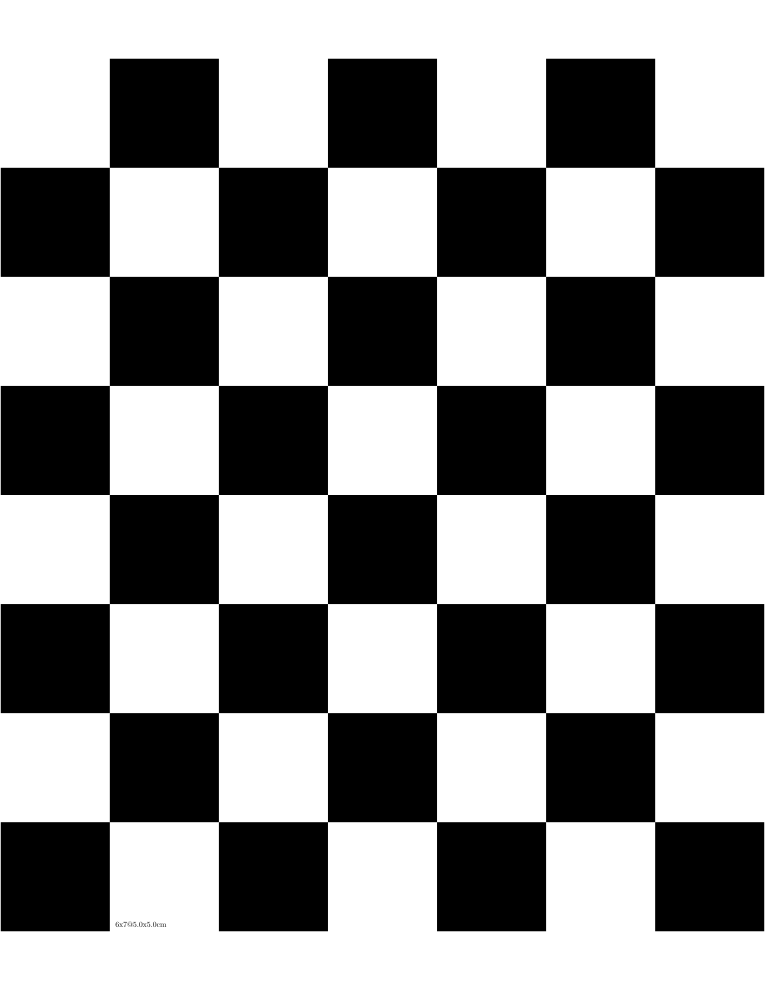
\includegraphics[width = 0.75\columnwidth]{Figures/checkerboard7x6x50x50cm.png}
		\caption[TOC Figure Name]{Title shown in text here: short paragraph description of picture here}
		\label{fig:examplePicture}
	\end{figure}

	Text description here, can reference other Chapters or Sections, like \Cref{ch:introduction} or \Cref{fig:examplePicture}.

\section{Radar Cross Section}
\label{sec:RCS}

An RCS encodes the expected angular response of a target in the presence of an electromagnetic wave. Radar cross sections are measured empirically, over multiple angles and frequencies.

\subsection[Optional TOC Subsection Title Here]{Subsection Title Here}
\label{sec:subsectionRefNameHere}
\phantomsection

Take about an equation with text without space, like
\begin{equation}
\label{eq:eqRefNameHere}
%\lambda
\frac{1}{z}
\begin{bmatrix}
u \\
v \\
1 \\
\end{bmatrix}=
K \begin{bmatrix}
x \\
y \\
z \\
\end{bmatrix}=
\begin{bmatrix}
f_x & 0 & c_x \\
0 & f_y & c_y \\
0 & 0 & 1 \\
\end{bmatrix}
\begin{bmatrix}
x \\
y \\
z \\
\end{bmatrix}
\end{equation}
where $\lambda$ can be referenced. Don't put lines before or after equations, unless the equation is the end of a paragraph's discussion.

You can also include an algorithm, like \Cref{alg:algorithmRefName}.

\begin{algorithm}[tb!]
	\caption{Algorithm Title Here}
	\label{alg:algorithmRefName}
	\begin{algorithmic}[1] % The number tells where the line numbering should start
		\Function{foo}{$a,b,c$}
		\State $\mathbf{R}^{C_0}_W,\mathbf{p}^W_{C_0} \gets \textsc{getPose}(e_0.t)$	\Comment{Target pose}
		\For{$k\gets 1,N$} \Comment{Loop over events}
		\State $\begin{bmatrix}x_H \\ y_H \end{bmatrix}  \gets \textsc{undistPos}(e_x,e_y)$ \Comment Pixel location to position
		\label{alg:line:lineRefName} % to use to reference specific lines in Algorithm
		\EndFor
		\State \textbf{return} $image$\Comment{Output}
		\EndFunction
	\end{algorithmic}
\end{algorithm}
